\chapter{三角関数}

{\small 過去の受講生の言葉: 「友人に教えてたら, 自分もわかっていなかったことに気づきました」}

\section{三平方の定理}

まず, 中学校で習った\underline{三平方の定理}
\index{さんへいほうのていり@三平方の定理} (ピタゴラスの定理)
\index{ぴたごらすのていり@ピタゴラスの定理}
を復習しておこう。\mv

\begin{q}\label{q:trig_Pitag} 三平方の定理を証明しよう。
直角三角形ABCを考える。角Cが直角であるとする。
点Cから辺ABに下ろした垂線の足を点Dとする。(図\ref{fig:Pitag})
\begin{enumerate}
\item 三角形ABCと三角形ACDは相似であることを示せ。
\item そのことから, AB:AC=AC:AD, すなわち\\
$\text{AB}\times \text{AD}=\text{AC}^2$であることを示せ。
\item 三角形ABCと三角形CBDは相似であることを示せ。
\item そのことから, AB:BC=BC:BD, すなわち\\
$\text{AB}\times \text{BD}=\text{BC}^2$であることを示せ。
\item 以上と$\text{AB}=\text{AD}+\text{BD}$より次式を示せ:
\begin{eqnarray}
\text{AB}^2=\text{AC}^2+\text{BC}^2\label{eq:pitagorus_0}
\end{eqnarray}
\end{enumerate}\end{q}
\begin{figure}[h]
    \centering
    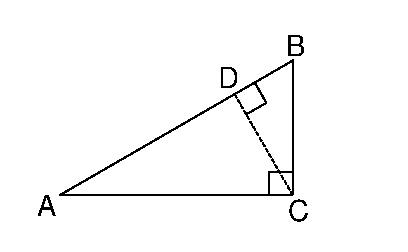
\includegraphics[width=5cm]{Pitag.eps}
    \caption{三平方の定理の証明に使う図}\label{fig:Pitag}
\end{figure}
\mv


\section{弧度法}

高校初年級までの数学や, 一般社会では, 角の大きさを「度」で表現することが多い。
「度」は, 一周を360度とする表現である。
360という数字と円の本質的な性質の間には, 数学的な必然性はない。たぶん, 子だくさんの家族で, 
丸いケーキを分ける時に, いろんな数で割り切れる360という数が好まれたのだろう!

角を「度」で表すときは, 細かい数字を小数で表す場合と, 
「分」「秒」という補助単位を使って表す場合(度分秒表記)がある。
60分=1度, 60秒=1分である。度, 分, 秒は, それぞれ°' "
という記号で表してもよい。例えば, 「36度6分42.5秒」は, 「36°6' 42.5"」と表す。

\begin{exmpl} 「36度6分42.5秒」という角を, 度だけで(分や秒を使わずに)表して
みよう。60秒=1分なので, 1秒=(1/60)分である。\\
従って, $42.5\text{秒}=42.5\times(1/60)\text{分}\fallingdotseq0.7083\text{分}$\\
従って, $6\text{分}42.5\text{秒}\fallingdotseq6+0.7083\text{分}=6.7083\text{分}$\\
また, 60分=1度なので, 1分=(1/60)度である。\\
従って, $6.7083\text{分}=6.7083\times(1/60)\text{度}\fallingdotseq0.11181\text{度}$\\
従って, $36\text{度}6\text{分}42.5\text{秒}\fallingdotseq36+0.11181\text{度}$\\$=36.11181\text{度}$。
\end{exmpl}

\begin{exmpl} 「140.10217度」という角を, 度分秒表記してみよう。
小数点以下の0.10217度は分や秒の単位で表されるはずだ。
1度=60分なので,\\
$\quad0.10217\text{度}=0.10217\times 60\text{分}=6.1302\text{分}$\\
となる。従って, 分の単位の値は6であり, 小数点以下の0.1302分は秒単位で表されるはずだ。従って,\\
$\quad0.1302\text{分}=0.1302\times 60\text{秒}=7.812\text{秒}$\\
従って, $140.10217\text{度}\fallingdotseq140\text{度}6\text{分}7.81\text{秒}$。
(例おわり)
\end{exmpl}
\mv

一方, 高校の上級(数II・数B以降)や大学の数学・物理学では, 以下で
定義される\underline{ラジアン}\index{らじあん@ラジアン} (radian)
という単位で角を表すことが多い:\hv

\textgt{半径1の円を切り取ってできる扇形において, その頂角を, 
扇形の弧の長さで表す(図\ref{fig:radian_illust})。
これを\underline{弧度法}\index{こどほう@弧度法}と呼ぶ。
弧度法での角度の単位を\underline{ラジアン}という。}

\begin{figure}[h]
    \centering
    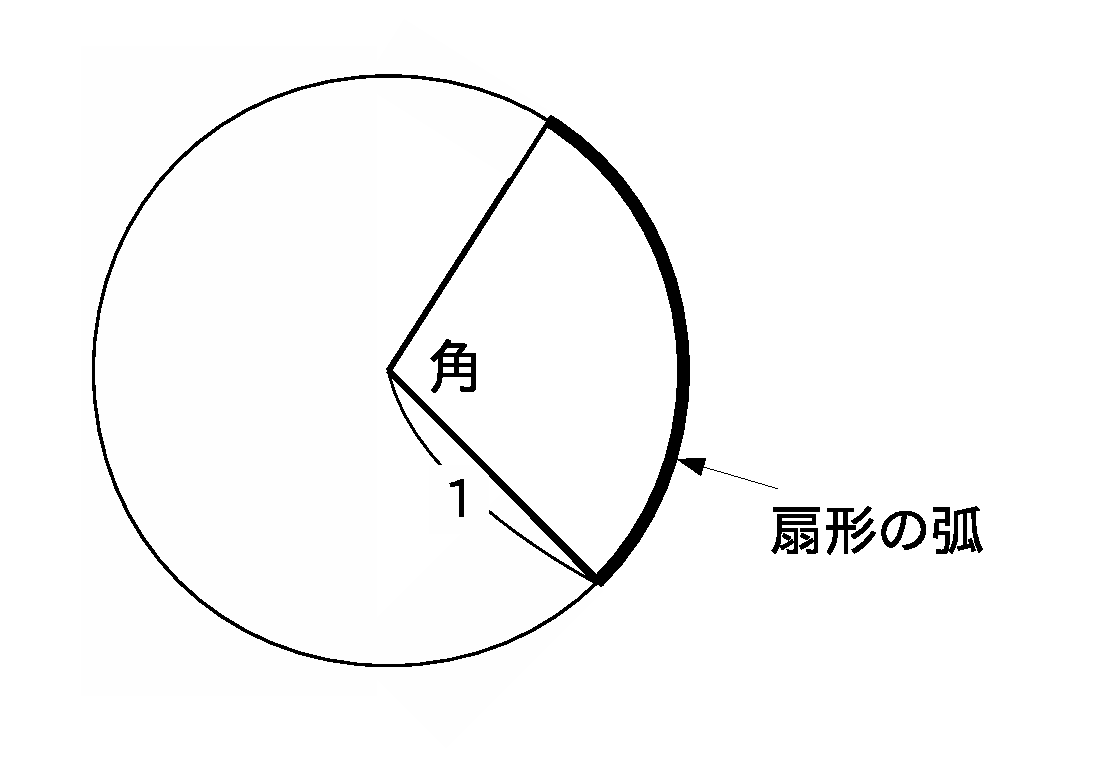
\includegraphics[width=6cm]{radian_illust.eps}
    \caption{弧度法}\label{fig:radian_illust}
\end{figure}

\begin{exmpl} 円を4つの扇型で等分すると, 1つの扇形の
頂角は90度。半径が1なら, その扇形の弧の長さは, 
$2\pi/4=\pi/2$。従って, $90\text{度}=\frac{\pi}{2}\text{ラジアン}$である。
\end{exmpl}

\begin{exmpl}\label{ex:2pi_360} 半径1, 中心角360度の「扇形」は, 円全体である。その「弧」は円周全体
だから, 長さは, $2\pi$である。従って, $360\text{度}=2\pi\text{ラジアン}$である。
(例おわり)\end{exmpl}\mv

弧度法(ラジアンで角度を表すこと)は, あまり直感的ではないが, 
数学的には自然である。後に学ぶが, 例えば, 弧度法では, 
三角関数をうまく微分できたり, 指数関数と三角関数を統一的に扱える。\hv

度からラジアンへの換算法を学ぼう: 半径1の円を切り取る扇形を
考えると, 扇形の頂角を度で表したものと弧長(ラジアン)は比例する。
従って度とラジアンは比例する。ところで例\ref{ex:2pi_360}
より, 360度は$2\pi$ラジアンなので, 
\begin{eqnarray}1\text{度}=\frac{2\pi}{360}\text{ラジアン}=\frac{\pi}{180}\text{ラジアン}\end{eqnarray}
となる。この式の左辺と右辺をそれぞれ$x$倍すれば, 
\begin{eqnarray}x\text{度}=\frac{\pi}{180}\,x\text{ラジアン}\label{eq:deg2rad}\end{eqnarray}
となる。また, この\eref{eq:deg2rad}の両辺を$180/\pi$倍して左辺と右辺を入れ替えれば, 
\begin{eqnarray}x\text{ラジアン}=\frac{180}{\pi}\,x\text{度}\label{eq:rad2deg}\end{eqnarray}
となる。\eref{eq:deg2rad}, \eref{eq:rad2deg}を使えば, 「度」とラジアンを相互に変換できる。\mv

ところで, 角度をラジアンで表記するときは, 多くの場合は, 慣習的に「ラジアン」という単位を省略する。
例えば, 「ある角は$\frac{\pi}{2}$ラジアンである」という記述は「ある角は$\frac{\pi}{2}$である」としてもよい。

\begin{faq}{\small\textgt{単位は省略してはダメじゃなかったんですか?} ... 
ラジアンの定義の中で, 「半径1」とあったでしょ? その1には単位はついていません。
つまり無次元量です。従って, この円の大きさは無次元量で表しています。
従って弧の長さも無次元量です。従って, 「$\frac{\pi}{2}$ラジアン」
は無次元量であり, 「ラジアン」という単位自体も無次元量なのです。本来, 
無次元量を表すのに単位は必要ありません。}
\end{faq}\mv

\begin{faq}{\small\textgt{うーん, よくわかりません} ... 
では, こう考えましょう。円の半径を$r$とし, 弧の長さを$l$とすると, 
$l/r$が, その扇型の頂角をラジアンで表したものになります。
ところが, $r$も$l$も「長さ」という次元の量なので, その比は
無次元量です。つまりラジアンで表した角は, 無次元量です。}
\end{faq}\mv


\begin{q}\label{q:trig_rad_def} 
角の大きさの表現法「ラジアン」を定義せよ。また, 「度」から「ラジアン」へ変換する式を示せ。
\end{q}\mv

\begin{q}\label{q:trig_deg2rad} 以下の角を, 「度」からラジアンへ変換せよ。
\begin{edaenumerate}<5>
\item 90°
\item 45°
\item 180°
\item 30°
\item 1°
\end{edaenumerate}\end{q}\hv

\begin{q}\label{q:trig_rad2deg} 以下の角を, ラジアンから「度」へ変換せよ。
\begin{edaenumerate}<5>
\item $\pi$
\item $\pi/3$
\item $2\pi$
\item $\pi/4$
\item 1
\end{edaenumerate}\end{q}
\mv

前問で, 1ラジアンは$180/\pi$度であることがわかった。$\pi$は約3なので, 
1ラジアンは約60度である($57.2957\cdots$度)。このことは, 弧度法の定義に
戻れば直感的に理解できる: 半径1で頂角1ラジアンの扇形では, 弧度法の定義によって, 
半径と弧長がともに1である。この扇形は, 
正三角形の1つの辺を円弧に変形したものと考えることもできるから, 頂角は
正三角形の角60度に近いだろう(図\ref{fig:1rad})。

\begin{figure}[h]
    \centering
    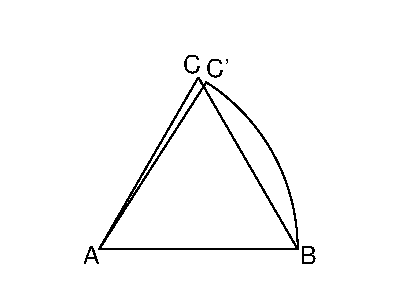
\includegraphics[width=5cm]{1rad.eps}
    \caption{1ラジアンの概念図。AB=BC=CA=1とする。正三角形ABCを少し歪ませると, 
扇形ABC'になる。辺BCと弧BC'は同じ長さ1である。角BACは$\pi/3$ラジアン(60度), 
角BAC'は1ラジアンである。この図から, 1ラジアンは60度に近い角であることが直感的に
理解できるだろう。}\label{fig:1rad}
\end{figure}
\mv

そもそも, 角は0以上2$\pi$以下なのだが, 数学では便宜上, 0未満や2$\pi$より
大きい角を考えたりする。そういう角は, $2\pi$を適当に足し引きして, 
0以上$2\pi$未満の範囲の角に帰着すればよい。例えば$3\pi$の角とは$2\pi+\pi$の角, 
つまり1周してさらに$\pi$回った角と考え, $2\pi$を余分とみなし, 
要するに$\pi$の角と同じ, と考える。

\begin{faq}{\small\textgt{なら, 要するに$3\pi=\pi$と書いていいのですか?}
... それは微妙です。もしそれが許されるなら, 両辺を2で割ってみましょう。
$3\pi/2=\pi/2$になっちゃいますね。度で言えば, この左辺は270度, 右辺は90度
です。変ですよね。だから, 「何周か余分に回った角」どうしを等号で
結ぶのは, やめておきましょう。}\end{faq}

\begin{q}\label{q:trig_rad2rad} 以下の角と同じになるような, 
0以上$2\pi$未満の角を述べよ。
\begin{edaenumerate}<3>
\item $-\pi$
\item $3\pi$
\item $-6\pi$
\end{edaenumerate}\end{q}
\mv

\begin{faq}{\small\textgt{ラジアンを定義せよという問題で, 「180度を$\pi$とする」と
書いたら不正解になりました。なぜ?}
... その解答では, 180度以外の角, たとえば90度とか20度とかについて定義
できないからダメなのです。\\
\textgt{でも, 90度は180度の半分だから, $\pi$の半分で$\pi/2$というふうに
解釈できると思います。}
... 度が半分になったらラジアンも半分になる, という定義は書かなかったでしょ? 
それが無いと, \pref{q:degC_K}の演習問題\ref{q:degC_K}のような変なことが
起きるかもよ!\\
\textgt{でも, このテキストでは一周を360度とする, と書いてありますよ。
半周や0.1周とかはどうなるのか, 度では定義できていないじゃないですか!}
... そうです。だからこのテキストは度でなくラジアンで話を進める
のです。度をきちんと定義したければ, まずラジアンを「単位円周を切り
とる弧の長さ」と定義し, ラジアンから度への換算式を書けばよいのです。}\end{faq}

\begin{freqmiss}{\small\textgt{角の大きさを, ラジアンで表してるのか
度で表してるのか混乱する} ... テキストの練習問題などでは, ラジアン表記
の角にはたいてい$\pi$が入っているので混乱しにくいですが, 
関数電卓やパソコンで計算する時は, ラジアンでも度でも, 一見, 
ただの数値ですので, この手のミスをしがちです。度で表す場合は
数値に必ず「度」か「°」をつけねばなりません。単位を忘れて単位を落とす!}\end{freqmiss}
\hv


\section{弧度法の応用: ビッターリッヒ法}\index{びったーりっひほう@ビッターリッヒ法}

%弧度法の考え方の応用例を紹介する。

\begin{q}\label{q:Bitterrich} 君は, 東南アジアの森林調査に出かけた。
すると, その森の材積量(単位面積あたり, どのくらいの体積の木質が蓄積されているか)
を推定するために, まず胸高断面積(人の胸のあたりの高さで木をぜんぶ切ったとして, 
その切口の面積の合計)を簡易的に推定するように依頼された。君は, 筑波大学で
習ったことを思い出し, 以下のような測定を行った。

まず君は, 森林内の1箇所に立ち, 片腕を水平に伸ばし, 親指を立てて, ぐるっと1回転しながら, 幹の太さが親指の陰に
隠れない木の本数$N$を数えた。片腕を水平に伸ばしたとき, 君の親指は, 君の水平方向の視角のうち$\theta$ラジアンをさえぎるとする。
君の親指の幅を$a$, 君の腕の長さを$l$とする。
\begin{enumerate}
\item $\theta \fallingdotseq a/l$であることを示せ。
\item 君の立ち位置から距離$R$にある, 胸高直径$d$の木の幹が, 君の親指にちょうどぴったり隠れるとき, 
\begin{eqnarray}d=R\theta\end{eqnarray}
であることを示せ。
\item 林の木は全て等しい胸高直径$d$を持つとしよう。上の式で決まる$R$よりも遠いところにある木は, 君の親指に隠れてしまう。このことから, 
$N$は君の立ち位置を中心とする半径$R=d/\theta$の円内の木の本数であることを示せ。
\item この円内の面積を$A$, この円内にある木の胸高断面積の合計を$B$とすると, 
\begin{eqnarray}
A&=&\pi R^2\\
B&=&N\pi d^2/4\end{eqnarray}
であることを示せ。ただし木の断面は全て円形であると仮定する。
\item この円内で, 単位面積あたりの胸高断面積は, 
\begin{eqnarray}\frac{B}{A}=\frac{N\theta^2}{4}\label{eq:Bitterrich_5}\end{eqnarray}
となることを示せ。
\item $a=2$ cm, $l=60$ cm, $N=10$のとき, 単位面積あたりの胸高断面積はどのくらいか? 
\item この方法は, どんな太さの木からなる林についても有効であることを示せ。
\item この方法は, さまざまな太さの木が混在する林についても有効であることを示せ。
\end{enumerate}
注:この方法は, 森林の胸高断面積を, 驚くほどの簡便さで推定する方法であり, 「ビッターリッヒ(Bitterlich)法」という。
一般に, 森林の材積量などを現場で正確に見積もるのは容易ではない。それを研究する分野を「森林計測学」という。
\end{q}
\hv

\section{三角関数}

半径1の円を\underline{単位円}\index{たんいえん@単位円} (unit circle)と呼ぶ。
\begin{figure}[h]
    \centering
    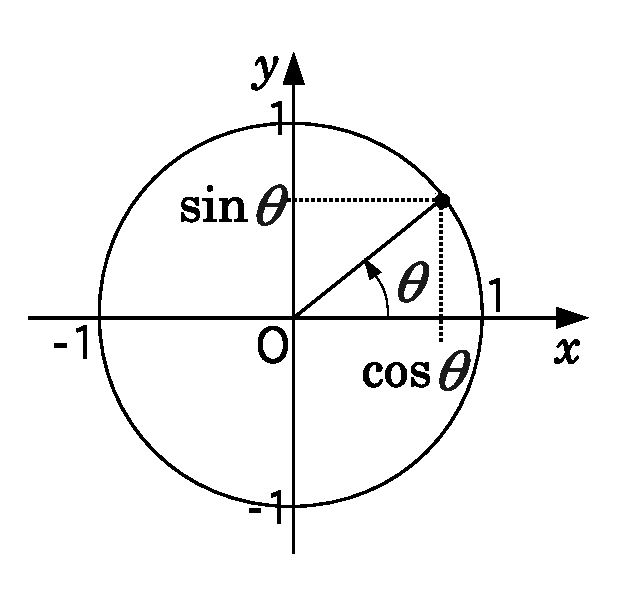
\includegraphics[width=6cm]{unit_circle.eps}
    \caption{単位円による, $\cos\theta$, $\sin \theta$の定義}\label{fig:unit_circle}
\end{figure}

\textgt{$xy$平面上で, 原点を中心とする単位円の上で, $(1, 0)$
から左回りに角$\theta$にある点の, $x$座標を$\cos \theta$, 
$y$座標を$\sin \theta$と定義する。
$\sin \theta / \cos \theta$を$\tan \theta$と定義する}(図\ref{fig:unit_circle})。

$\cos \theta$, $\sin \theta$, $\tan \theta$のことを, 
\underline{三角関数} \index{さんかくかんすう@三角関数}
(trigonometry)と呼ぶ。
$\cos$\index{cos}は「コサイン」, $\sin$\index{sin}は「サイン」, $\tan$\index{tan}は
「タンジェント」と読む。コサインを「余弦」\index{よげん@余弦}, 
サインを「正弦」\index{せいげん@正弦}, タンジェントを「正接」\index{せいせつ@正接}
と呼ぶこともある。\mv

\begin{q}\label{q:trig_unitC} 単位円とは何か?\end{q}

\begin{q}\label{q:trig_sincos_def} 
角$\theta$について, $\cos \theta$, $\sin \theta$, $\tan \theta$のそれぞれを定義せよ。\end{q}

\begin{faq}{\small\textgt{上の問題で, 「単位円上の
点の$x$座標を$\cos\theta$, $y$座標を$\sin\theta$, $\sin\theta/\cos\theta$を
$\tan\theta$という, と書いたら不正解になりました。なぜ?}
... その答案では$\theta$が何にあたるのか明言されていないからです。}\end{faq}

\begin{q}\label{q:trig_sincos2} 
$\cos \theta$や$\sin \theta$は, 全ての実数$\theta$について$-1$から1の範囲の値
をとることを示せ。ヒント:単位円の上の点の座標はどのような範囲を動くか? \end{q}

\begin{q}\label{q:trig_sincos6} 
以下の角$\theta$について, 正弦\index{せいげん@正弦} ($\sin \theta$のこと), 余弦
\index{よげん@余弦} ($\cos \theta$のこと), 正接\index{せいせつ@正接} 
($\tan \theta$のこと)の値をそれぞれ求めよ(表にせよ)。最後の4問は, 関数電卓を使う。
(14)(15)(16)の単位はラジアン。
\begin{edaenumerate}<4>
\item 0°
\item 30°
\item 45°
\item 60°
%\item 75°
\item 90°
\item 120°
%\item 150°
\item 180°
\item 270°
\item $-30$°
\item $\pi/6$
\item $\pi/4$
\item $\pi/3$
\item 1°
\item 1
\item 0.1
\item 0.01
\end{edaenumerate}\end{q}
{\small 注: 関数電卓で三角関数を計算するときは, その関数電卓が角を「ラジアン」
で解釈するのか「度」で解釈するのか, どちらのモードにあるのかを確認する必要がある。
画面の端っこに, RADとかRという表示が小さく出ているならおそらくラジアンモードだし, 
DEGとかDという表示が小さく出ているなら, おそらく度モードである。確認する
には, 90を与えて$\sin$を計算させてみることである。その結果が1ならば度モード
だし, 1以外の数値($0.893\cdots$)ならばラジアンモードだ。多くの関数電卓は, 
これらのモードを切り替えることができる。\pref{fig:calculator}の図\ref{fig:calculator}
の左上あたりのように, 多くの関数電卓には, shiftというキーとMODEというキーがある。
これらを使って切り替えるのだ。そのやりかたはそれぞれ関数電卓によって異なるので, 
いろいろ試してみよう。どうしても切り替え方がわからなければ, 
\eref{eq:deg2rad}や\eref{eq:rad2deg}を使ってラジアンと度を
変換して計算すればよい。}
\mv

前問の(15), (16)の経験から, ラジアンで表現すれば, $\theta$が0に近ければ近いほど, 
\begin{eqnarray}
\sin \theta \fallingdotseq \theta \,\,\, \text{かつ, }\,\,\, \tan \theta \fallingdotseq \theta
\label{eq:sinx_x}
\end{eqnarray}
であることがわかるだろう。
%このことは, 後で三角関数の微分を考える時に登場するので, 頭の片隅に入れておこう。
\mv

ちなみに, あまり使わないが, $\cos$と$\sin$の逆数には, sec\index{sec} (セカント)と
cosec\index{cosec} (コセカント)という名前がついている:
\begin{eqnarray}
\text{sec}\, \theta:=\frac{1}{\cos \theta},\,\,\,\,\,\text{cosec}\, \theta:=\frac{1}{\sin \theta}
\end{eqnarray}
\mv

\section{三角関数の公式}

三角関数には以下のように, たくさん公式(定理)がある。
それらを覚えるのが嫌で, 三角関数苦手!という人も多いが, 
定義に戻れば簡単にわかることばかりであり, 無理に暗記するものではない。
忘れてもその場で自力で証明すればいいのだ。以下, $\theta$を
任意の角とする。

まず, 次の式が成り立つ:
\begin{eqnarray}
\cos ^2 \theta + \sin ^2 \theta = 1\label{eq:trig_cos2_sin2_1}
\end{eqnarray}
なぜか? 原点から点$(\cos\theta,\, \sin\theta)$までの距離は, 
三平方の定理から, $\sqrt{\cos^2\theta+\sin^2\theta}$。一方, 
定義より$(\cos\theta,\, \sin\theta)$で表される点は単位円上にあるので, 
原点からの距離は1。従って, $\sqrt{\cos^2\theta+\sin^2\theta}=1$。
両辺を2乗すると\eref{eq:trig_cos2_sin2_1}を得る。\\

角は$2\pi$ラジアンでひとまわりなので, $\theta$と$\theta+2\pi$は
同じ角を意味する。従って, 次の2つの式が成り立つ:
\begin{eqnarray}
\cos (\theta+2\pi) = \cos \theta\label{eq:trig_sincos3_q1}\\
\sin (\theta+2\pi) = \sin \theta\label{eq:trig_sincos3_q2}
\end{eqnarray}
すなわち, $\sin$や$\cos$は, $2\pi$ごとに, 同じ値が繰り返し
出てくるのだ。\mv

さて, \fref{fig:unit_circle2}のように, $-\theta$という角は, 
$x$軸から逆まわり(右回り; 時計回り)に$\theta$だけ回った角である。
それは, $\theta$という角($x$軸から左回りで回った角)とは, 
$x$軸に関して対称の位置にある。
\begin{figure}[h]
    \centering
    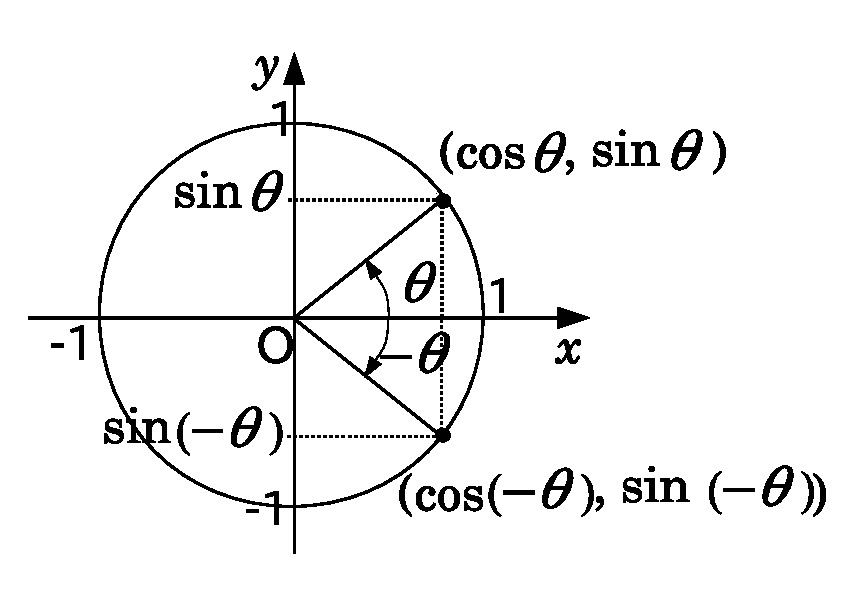
\includegraphics[width=7cm]{unit_circle2.eps}
    \caption{\eref{eq:trig_cos_even}, \eref{eq:trig_sin_odd}を示す図}\label{fig:unit_circle2}
\end{figure}
従って, 
$(\cos(-\theta), \sin(-\theta))$と$(\cos\theta, \sin\theta)$
は, $x$軸に関して対称の位置にある(\fref{fig:unit_circle2})。
すなわち, $x$座標は同じで$y$座標は正負が逆。従って, 次の2つの式が成り立つ:
\begin{eqnarray}
&&\cos (-\theta) = \cos \theta\label{eq:trig_cos_even}\\
&&\sin (-\theta) = - \sin \theta\label{eq:trig_sin_odd}
\end{eqnarray}

これらと同様に, 次の問の各式を証明できる。コツは, 面倒でも毎回, 
\fref{fig:unit_circle2}みたいな図を描き, 単位円上での点の
位置関係(対称性)を使うことである。

\begin{q}\label{q:trig_sincos3} $n$を整数とする。三角関数の定義から, 以下の式を導け。
\begin{eqnarray}
&&\cos (\pi - \theta) = - \cos \theta\\
&&\sin (\pi - \theta) = \sin \theta\\
&&\cos (\pi + \theta) = - \cos \theta\\
&&\sin (\pi + \theta) = - \sin \theta\\
&&\cos \Bigl(\frac{\pi}{2} - \theta\Bigr) = \sin \theta\label{eq:trig_cosx_2pi}\\
&&\sin \Bigl(\frac{\pi}{2} - \theta\Bigr) = \cos \theta\label{eq:trig_sinx_2pi}\\
&&\cos \Bigl(\frac{\pi}{2} + \theta\Bigr) = -\sin \theta\\
&&\sin \Bigl(\frac{\pi}{2} + \theta\Bigr) = \cos \theta\label{eq:trig_sinx_plus_pi2}
\end{eqnarray}
ヒント: $\pi-\theta$は, $\theta$とは$y$軸対称。$\pi+\theta$は, $\theta$とは原点対称。
$\pi/2-\theta$は, $\theta$とは$x$軸と$y$軸を入れ替えた関係(直線$y=x$に関して対称)。
言い換えれば, $y$軸から右周り(時計回り)に$\theta$だけ回った角。$\pi/2+\theta$は, 
$y$軸から左周り(反時計回り)に$\theta$だけ回った角。
\end{q}

\begin{q}\label{q:trig_sincos4} $n$を整数とする。三角関数の定義から, 以下の式を導け。
\begin{eqnarray}
&&\sin n\pi=0\label{eq:trig_sinpix}\\
&&\cos n\pi=(-1)^n\label{eq:trig_cospix}
\end{eqnarray}
\end{q}

\begin{q}\label{q:trig_tan} 三角関数の定義から, 以下の式を導け。
\begin{eqnarray}
&&1+\tan^2 \theta = \frac{1}{\cos^2\theta}\\
&&\tan(-\theta) = -\tan\theta\label{q:trig_tan_minus}\\
&&\tan(\theta+\pi) = \tan\theta\label{q:trig_tan_period}
\end{eqnarray}\end{q}
\mv

ここで\eref{q:trig_tan_period}に注意しよう。これを見ると, 
$\tan$は, $\theta$が$\pi$増えるごとに, 同じ値が繰り返し
出てくるのだ。$\sin$や$\cos$は$2\pi$ごとの繰り返しだったが, 
$\tan$はその半分で繰り返しが来るのだ。このことは, あとで$\tan$の
グラフを見れば, よりはっきりわかるだろう。\mv


\begin{q}\label{q:trig_evenodd} $\cos\theta$, $\sin\theta$, $\tan\theta$は, 
それぞれ, $\theta$の関数と見たとき, 偶関数? 奇関数? あるいはそのどちらでもない?
\end{q}
\mv


\section{加法定理}

次に述べるのは, 2つの角の和の三角関数を, それぞれの角の三角関数で
表す公式であり, 「加法定理」と呼ばれる。三角関数の応用では頻繁に
出てくる, 重要な定理である。

\begin{q}\label{q:trig_kahouteiri} 単位円の上に, $x$軸から角$\alpha$だけ
離れたところに点Aをとり, $x$軸から角$-\beta$だけ離れたところに点Bをとる。
このとき, 原点Oと点A, 点Bを頂点とする三角形OABを考える。一方, 単位円と
$x$軸が交わる点(1, 0)をA'とし, 単位円上で$x$軸から角$\alpha+\beta$だけ
離れたところに点B'をとる。このとき, 原点Oと点A', 点B'を頂点
とする三角形OA'B'を考える。
\begin{enumerate}
\item 三角形OABと三角形OA'B'をそれぞれ別の図として作図せよ。
\item 三角形OABと三角形OA'B'が合同であることを示せ。
\item 点A, 点Bの各座標を, $\alpha, \beta$を用いて表せ。
\item 辺ABの長さの2乗(AB$^2$)を, $\alpha, \beta$を用いて表せ。
\item 点A', 点B'の各座標を, $\alpha, \beta$を用いて表せ。
\item 辺A'B'の長さの2乗(A'B'$^2$)を, $\alpha, \beta$を用いて表せ。
\item AB$^2=$A'B'$^2$より, 次式を示せ。
\begin{eqnarray}
\cos(\alpha + \beta)=\cos\alpha \cos\beta - \sin\alpha \sin\beta\label{eq:add_sin1}
\end{eqnarray}
\item \eref{eq:trig_cosx_2pi}より$\sin(\alpha + \beta)=\cos(\pi/2-\alpha - \beta)$
が成り立つ。このことを利用して, 次式を示せ:
\begin{eqnarray}
\sin(\alpha + \beta)=\sin\alpha \cos\beta + \cos\alpha \sin\beta\label{eq:add_sin2}
\end{eqnarray}
ヒント: $\sin(\alpha + \beta)$を$\cos((\pi/2-\alpha) + (-\beta))$と考え, \eref{eq:add_sin1}を使う。
\end{enumerate}\end{q}
\eref{eq:add_sin1}と\eref{eq:add_sin2}は, $\alpha, \beta$がどのような角であっても成り立つ。
これらの式を三角関数の\underline{加法定理} \index{かほうていり@加法定理}と呼ぶ。

加法定理の特別な場合として, 以下のような公式が成り立つ。

\begin{q}\label{q:trig_kahouteiri2} 以下の式を示せ\index{ばいかくこうしき@倍角公式}:
\begin{eqnarray}
&&(1)\,\,\,\,\cos(\alpha - \beta)=\cos\alpha \cos\beta + \sin\alpha \sin\beta\,\,\,\,\,\,\,\,\,\,\,\,\,\,\,\,\,\,\,\,\,\,\,\,\,\,\,\,\,\,\,\,\,\label{eq:add_sin3}\\
&&(2)\,\,\,\,\sin(\alpha - \beta)=\sin\alpha \cos\beta - \cos\alpha \sin\beta\,\,\,\,\,\,\,\,\,\,\,\,\,\,\,\,\,\label{eq:add_sin4}\\
&&(3)\,\,\,\,\text{(cosの倍角公式)}\nonumber\\
&&\,\,\,\,\,\,\,\,\,\,\,\,\cos 2\alpha = \cos^2 \alpha - \sin^2 \alpha \label{eq:cos2_1}\\
&&\,\,\,\,\,\,\,\,\,\,\,\,\,\,\,\,\,\,\,\,= 2\cos^2 \alpha - 1 \label{eq:cos2_2}\\
&&\,\,\,\,\,\,\,\,\,\,\,\,\,\,\,\,\,\,\,\,= 1 - 2\sin^2 \alpha \label{eq:cos2_3}\\
&&(4)\,\,\,\,\text{(sinの倍角公式)}\nonumber\\
&&\,\,\,\,\,\,\,\,\,\,\,\,\sin 2 \alpha = 2 \sin \alpha \cos \alpha\label{eq:sin2a}
\end{eqnarray}
\end{q}

\begin{q}\label{q:trig_sincos5} 以下の式を示せ:
\begin{eqnarray}
&&(1)\,\,\,\,\,\cos^2 \alpha = \frac{1+\cos 2\alpha}{2}\label{eq:cos_pow2}\\
&&(2)\,\,\,\,\,\sin^2 \alpha = \frac{1-\cos 2\alpha}{2}\label{eq:sin_pow2}
\end{eqnarray}
\end{q}
\mv

\eref{eq:add_sin1}〜\eref{eq:sin_pow2}は, いずれも重要な公式なので, 
少なくとも, 自力で導出できるようになろう。できれば覚えることが望ましい
(数IIIを受験で使った人は覚えたはず!)。少しくらい忘れても, うろおぼえの状態
から正しい式を思い出すコツがある。\mv

\begin{exmpl}
\eref{eq:add_sin1}〜\eref{eq:add_sin4}
を混同してしまい, 右辺の符号($\pm$)や$\sin$と$\cos$の順序を間違えることがよくある。そんなときは, $\alpha=\beta=0$
とか, $\alpha=0, \beta=\pi/2$などの値を代入して, 左辺と右辺が整合的になるかどうかを確かめればよい。例えば, 
\[\cos(\alpha + \beta)=\sin\alpha \sin\beta - \cos\alpha \cos\beta \cdots\text{(これは間違い)}\]
だったっけ? と考える。ここで$\alpha=\beta=0$を代入すると, 左辺は1, 右辺は$-1$になるから, 何かが違う!なら, 
\[\cos(\alpha + \beta)=\sin\alpha \cos\beta - \cos\alpha \sin\beta \cdots\text{(これも間違い)}\]
かな? と考える。ここで$\alpha=\beta=0$を代入すると, 左辺は1, 右辺は$0$になるから, やっぱり何かが違う!そうやって, 
可能性を絞り込んで行くことができる。
\end{exmpl}\mv

\begin{exmpl}
\eref{eq:trig_cosx_2pi}を忘れたら, \eref{eq:add_sin1}を用いて導出できる:
\begin{eqnarray*}
\cos \Bigl(\frac{\pi}{2} - \theta\Bigr) = \cos\frac{\pi}{2}\cos\theta+\sin\frac{\pi}{2}\sin\theta
\end{eqnarray*}
ここで, $\cos(\pi/2)=0$, $\sin(\pi/2)=1$より, 上の式の右辺は, $\sin \theta$となる。(例おわり)
\end{exmpl}\mv



\section{三角関数のグラフ}

次に, $y=\sin x$や$y=\cos x$等のグラフを描けるようになろう。
$y=\sin x$のグラフは図\ref{fig:sin}である。
\begin{figure}[h]
    \centering
    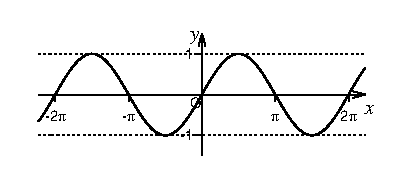
\includegraphics[width=6.5cm]{sin.eps}
    \caption{$y=\sin x$のグラフ}\label{fig:sin}
\end{figure}

このグラフには, 関数$y=\sin x$の, 次のような性質がよくあらわれている:
\begin{itemize}
\item $\sin 0=0$
\item $x$が$2\pi$だけ進むと, もとの値に戻る。
\item $y$は$-1$から$1$までの範囲の値だけをとる。
\item $x=\pi/2$のとき(直角のとき), 最大値1をとる。
\item 奇関数である。
\end{itemize}

\fref{fig:sin}は波っぽい形のグラフである。そこで, このような
形(\fref{fig:sin}を拡大縮小したり平行移動した形)を
「正弦曲線」\index{せいげん曲線@正弦曲線}という。

次に$y=\cos x$のグラフを描こう。\eref{eq:trig_sinx_plus_pi2}から, 
\begin{eqnarray}\sin\Bigl(x+\frac{\pi}{2}\Bigr)=\cos x\end{eqnarray}
だから, $y=\sin x$のグラフを左に($x$軸の負の方向に)$\pi/2$だけ
平行移動したものが$y=\cos x$のグラフになる。従って図\ref{fig:cos}のようになる。
$\cos x$が偶関数であることが, きちんと表現されている。\hv
\begin{figure}[h]
    \centering
    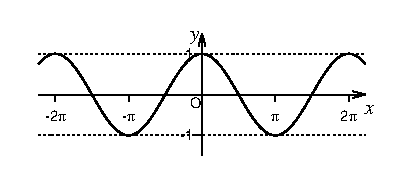
\includegraphics[width=6.5cm]{cos.eps}
    \caption{$y=\cos x$のグラフ}\label{fig:cos}
\end{figure}
このグラフは\fref{fig:sin}のグラフを平行移動したものとみなせるから, 
正弦曲線と言える(余弦なのに!?)。

次に$y=\tan x$のグラフを描こう。まず, 定義より
\begin{eqnarray}
\tan x=\frac{\sin x}{\cos x}
\end{eqnarray}
だから, $\tan x$は奇関数であり, $x=0$のときに0をとることがすぐわかる。
また, $x$が0から次第に増加すると, 最初のうちは$\sin x$は増加, $\cos x$は
減少するから, $\tan x$は次第に増加する。$x=\pi/2$に近づくと, 分母の
$\cos x$が0に近づくから, $\tan x$の値はどんどん大きくなって$\infty$に飛んでいく。
ところが$x=\pi/2$を少し越えると, $\cos x$は0に近いマイナスの値になり, 
$\sin x$はプラスの値のままだから, $\tan x$の値は, いきなり$-\infty$に飛んで行ってしまう。

そういうふうに考えると, $y=\tan x$のグラフが図\ref{fig:tan}のようになることが, 納得できるだろう:
\begin{figure}[h]
    \centering
    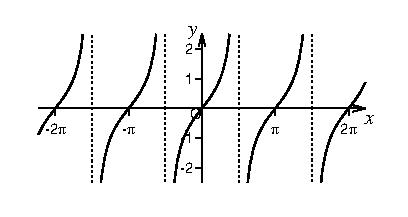
\includegraphics[width=6.5cm]{tan.eps}
    \caption{$y=\tan x$のグラフ。点線は漸近線。}\label{fig:tan}
\end{figure}

\begin{q}\label{q:trig_singraph0} 以下の関数のグラフをひとつに重ねて描け。
\begin{edaenumerate}
\item $y=\sin x$
\item $y=\cos x$
\item $y=\tan x$
\item $y=\sin 2x$
\end{edaenumerate}\end{q}

\begin{q}\label{q:trig_singraph1} $y=\sin^2 x$のグラフを書いてみよう。
\begin{enumerate}
\item $y$は常に0以上, つまり$x$軸よりも上にあることを示せ。
\item $y$は1よりも大きくはならないことを示せ。
\item このグラフは原点を通ることを示せ。
\item このグラフは$y$軸に関して対称(偶関数)であることを示せ。
\item 式(\ref{eq:sin_pow2})も参考にして, この関数のグラフを描け。
\end{enumerate}\end{q}
\begin{figure}[h]
    \centering
    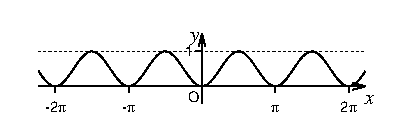
\includegraphics[width=7cm]{sin_square.eps}
    \caption{$y=\sin^2 x$のグラフ\label{fig:sin_square}。$x$軸に接する部分がなめらかな曲線になっていることに注意。}
    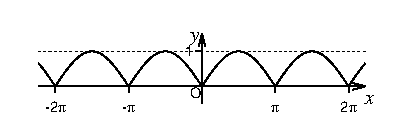
\includegraphics[width=7cm]{sin_abs.eps}
    \caption{$y=|\sin x|$のグラフ。この図は図\ref{fig:sin}つまり$y=\sin x$のグラフの$x$軸より下の
部分を上に折り返したものでもある。従って, $x$軸に接する部分はとがっている。図\ref{fig:sin_square}との
違いをじっくり観察しよう。\label{fig:sin_abs}}
\end{figure}

\begin{freqmiss}{\small\textgt{$y=\sin^2 x$のグラフを描けと言われて, 
図\ref{fig:sin_abs}のようなグラフを描いてしまう。}}\end{freqmiss}
\vv



\section{三角形と三角関数}

以上は「三角関数」の話なのに三角形が登場せず, 円ばかり
出てきた。そう, 実は, 「三角関数」は三角形の関数よりも
むしろ円の関数なのだ。それが「三角関数」と呼ばれる
のは歴史的な経緯にすぎない。しかし, 三角形と三角関数の関係も重要である。\mv

\begin{q}\label{q:trig_triang_sincos0} 図\ref{fig:triangle_rect}の直角三角形OABについて, 
次式を示せ:
\begin{eqnarray}
&\text{(1) }\,\,\,\, \sin \theta&=\frac{\text{AB}}{\text{OA}}\label{eq:trig_defclassic_sin}\\
&\text{(2) }\,\,\,\, \cos \theta&=\frac{\text{OB}}{\text{OA}}\label{eq:trig_defclassic_cos}\\
&\text{(3) }\,\,\,\, \tan \theta&=\frac{\text{AB}}{\text{OB}}\label{eq:trig_defclassic_tan}
\end{eqnarray}\end{q}
\begin{figure}[h]
    \centering
    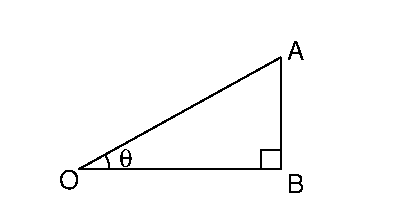
\includegraphics[width=5cm]{triangle_rect.eps}
    \caption{問\ref{q:trig_triang_sincos0}の説明図}\label{fig:triangle_rect}
\end{figure}

高校の数学IIでは, \eref{eq:trig_defclassic_sin}, \eref{eq:trig_defclassic_cos}, 
\eref{eq:trig_defclassic_tan}を利用して三角関数を定義している。しかし, これらは$\pi/2$
以上の角や負の角には適用できないので, 大学レベルの数学では三角関数を単位円で定義するのだ。

\begin{freqmiss}{\small\textgt{sinやcosを, いつまでも直角三角形の辺の比で定義する} ... 
間違いとまでは言えないけど, それは一般性に欠ける不完全な定義です。
単位円を使おう。}\end{freqmiss}

実用的には, \eref{eq:trig_defclassic_sin}, \eref{eq:trig_defclassic_cos}, 
\eref{eq:trig_defclassic_tan}は, 以下のような形で使われることが多い。
\begin{eqnarray}
\text{AB}=\text{OA}\,\sin \theta\label{eq:trig_defclassic_sin1}\\
\text{OB}=\text{OA}\,\cos \theta\label{eq:trig_defclassic_cos1}\\
\text{AB}=\text{OB}\,\tan \theta\label{eq:trig_defclassic_tan1}
\end{eqnarray}

\begin{q}\label{q:trig_triang_sincos1} 傾斜30度の斜面を, 斜距離で100 mだけ登ると, 高度は約何mだけ上がるか? 
\end{q}\mv

\begin{q}\label{q:trig_triang_sincos2} 傾斜3度の斜面を, 斜距離で100 mだけ登ると, 高度は約何mだけ上がるか? 
3度を0に近い量とみなし, 式(\ref{eq:sinx_x})を使って近似計算してみよ。
\end{q}\mv

\section{正弦定理と余弦定理}

ここで, 三角形の辺と角の間に成り立つ重要な定理を2つ, 学ぶ。
これらは, 生物資源学類では, 森林や農地の測量に必要である。

\begin{figure}[h]
    \centering
    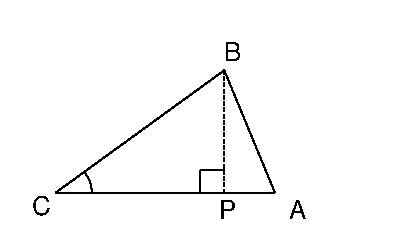
\includegraphics[width=5cm]{triangle_sincos.eps}
    \caption{問\ref{q:trig_yogen}の説明図}\label{fig:triangle_sincos}
\end{figure}

\begin{q}\label{q:trig_seigen} 
図\ref{fig:triangle_sincos}のような三角形ABCを考える。
BCの長さを$a$, CAの長さを$b$, ABの長さを$c$とする。
頂点A, B, Cをそれぞれ挟む角の大きさをそれぞれ$A, B, C$
とする(例えば角ACBの大きさが$C$)。
%簡単のため, これは鋭角三角形(つまり, $A, B, C$は全て鋭角)とする。
Bから辺CAにおろした垂線の足をPとする。
\begin{enumerate}
\item 次式を示せ。
\begin{eqnarray}
\text{BP}=a\sin C
\end{eqnarray}
\item 三角形ABCの面積を$S$とする。次式を示せ。
\begin{eqnarray}
S=\frac{a\,b\sin{C}}{2}\label{eq:triangle_area1}
\end{eqnarray}
\item 同様に考えて次式を示せ。
\begin{eqnarray}
S=\frac{b\,c\sin{A}}{2}\label{eq:triangle_area22}\\
S=\frac{c\,a\sin{B}}{2}\label{eq:triangle_area23}
\end{eqnarray}
\item \eref{eq:triangle_area1}〜\eref{eq:triangle_area23}から次式を示せ:
\begin{eqnarray}
\frac{a}{\sin A}=\frac{b}{\sin B}=\frac{c}{\sin C}\label{eq:trig_seigen}
\end{eqnarray}
\end{enumerate}
\end{q}

\eref{eq:trig_seigen}を\underline{正弦定理} \index{せいげんていり@正弦定理}と呼ぶ。\mv

\begin{q}\label{q:trig_yogen}
前問の続きを考える。
\begin{enumerate}
\item CP=$a\cos C$, AP=$|b-a\cos C|$となることを示せ。
\item 直角三角形PABについて三平方の定理を考えて, 次式を示せ:
\begin{eqnarray}
c^2=(a\sin C)^2+(b-a\cos C)^2
\end{eqnarray}
\item 前小問より, 次式を示せ:
\begin{eqnarray}
c^2=a^2+b^2-2ab\cos C\label{eq:th_cos1}
\end{eqnarray}
\end{enumerate}\end{q}\mv

この問題で, 三角形ABCの頂点と辺の名前付けを適当に変えると, 以下の式も成り立つ:
\begin{eqnarray}
a^2=b^2+c^2-2bc\cos A\label{eq:th_cos12}\\
b^2=c^2+a^2-2ca\cos B\label{eq:th_cos13}
\end{eqnarray}

また, \eref{eq:th_cos1}〜\eref{eq:th_cos13}を少し変形すると次式が成り立つ:
\begin{eqnarray}
\cos C=\frac{a^2+b^2-c^2}{2ab}\label{eq:th_cos2}\\
\cos A=\frac{b^2+c^2-a^2}{2bc}\label{eq:th_cos3}\\
\cos B=\frac{c^2+a^2-b^2}{2ca}\label{eq:th_cos4}
\end{eqnarray}

\eref{eq:th_cos1}〜\eref{eq:th_cos4}を\underline{余弦定理}
\index{よげんていり@余弦定理}と呼ぶ。

\begin{q}\label{q:trig_yogen_pyutag}
\eref{eq:th_cos1}は, 角Cが直角の場合, 三平方の定理に一致することを示せ。\end{q}

このように, 余弦定理は, その特別な場合として三平方の定理を含んでいる。いわば, 
三平方の定理の拡張版である。
\mv

\begin{faq}{\small\textgt{\eref{eq:th_cos1}〜\eref{eq:th_cos4}は
全部覚えるべきですか?} ... どれか1つだけでいいので, 何も見ないで
導出できるくらい何回も証明してみましょう。そうすれば, 忘れても自力で
導出できるし, 残りは全部, そこから記号の置き換えと式変形で
出てきます。}\end{faq}
\mv

さて, 多角形の面積を求める時, 多角形を三角形に分割し, 
それぞれの三角形の面積を求めて足す, ということがよく行われる。
その際, 最も基本的なのは, 「3辺の長さがわかっている三角形の
面積を求めよ」という問題だ。

\begin{q}\label{q:trig_area} 3辺の長さがそれぞれ
$a=4\,$cm, $b=3\,$cm, $c=2\,$cmである三角形の面積を求めてみよう。$\theta$を, $a$と$b$の各辺に挟まれた角とする。
\begin{enumerate}
\item 式(\ref{eq:th_cos2})から$\cos\theta$の値を求めよ。
\item $\cos^2\theta+\sin^2\theta=1$から, $\sin\theta$の値を求めよ。
\item 式(\ref{eq:triangle_area1})から, この三角形の面積を求めよ。
\end{enumerate}\end{q}

{\small 注: 三角形の面積に関する「ヘロンの公式」というものがあり, それを使って
問\ref{q:trig_area}を解く人がたまにいるが, その場合は, ヘロンの公式を
証明することが必要である。率直に言えば, ヘロンの公式は煩雑なだけで, あまり
便利なものではない。\eref{eq:triangle_area1}と余弦定理の組み合わせで十分に
代用できる。}

\begin{freqmiss}{\small\textgt{問\ref{q:trig_area}(3)の答に単位をつけない} ... 
当然, 不正解です。}\end{freqmiss}
\vv



\section{逆三角関数}\label{sec:arcsin}
\index{ぎゃくさんかくかんすう@逆三角関数}

cos, sin, tanのそれぞれの逆関数を, 
$\arccos$\index{arccos} (アークコサイン\index{あーくこさいん@アークコサイン}), 
$\arcsin$\index{arcsin} (アークサイン\index{あーくさいん@アークサイン}), 
$\arctan$\index{arctan} (アークタンジェント\index{あーくたんじぇんと@アークタンジェント})
と呼ぶ。 これらを逆三角関数という。\hv

ただし, この定義はまだ不完全である。というのも, 
例えば$\cos \theta=1/2$となるような$\theta$をarccos(1/2)というのだが, 
cosは周期的な関数なので, $\cos \theta=1/2$となるような$\theta$の値は, 
$\pm\pi/3$や$\pm7\pi/3$や$\pm13\pi/3$など, たくさんあるから, 
どれなのか迷ってしまう。そこで, arccosの値は, $0$以上$\pi$以下
に限定するのだ。すなわち, \\
「$\arccos x$とは, $\cos \theta=x$かつ$0\leq\theta\leq\pi$
となるような$\theta$のことである」\\
と定義する。従って, 例えば
\begin{eqnarray}
\arccos\frac{1}{2}=\frac{\pi}{3}
\end{eqnarray}
である($-\pi/3$や$7\pi/3$などはこの答に含めてはいけない)。

同様に, \\
「$\arcsin x$とは, $\sin \theta=x$かつ$-\pi/2\leq\theta\leq\pi/2$
となるような$\theta$のことである」\\
「$\arctan x$とは, $\tan \theta=x$かつ$-\pi/2\leq\theta\leq\pi/2$
となるような$\theta$のことである」\\
と定義する。\hv

{\small 注1: $\arcsin$と$\arctan$は, $\arccos$とは値域($\theta$のとり得る
範囲)が違うことに注意せよ。

注2: $\arcsin x$をArcsin $x$とか$\sin^{-1} x$と書くこともある。後者の
場合は$1/\sin x$と間違えないように。同様に, $\arccos x$をArccos $x$
とか$\cos^{-1}x$と書くこともある。後者の場合は$1/\cos x$と間違えないように。
同様に, $\arctan x$をArctan $x$とか$\tan^{-1}x$と書くこともある。後者の
場合は$1/\tan x$と間違えないように。

注3: $\theta$がどんな値であっても$\cos\theta$と$\sin\theta$は
$-1$以上1以下の値しか取り得ない。従って, $x$が1より大きかったり$-1$より
小さかったりする場合は, $\sin\theta=x$とか$\cos\theta=x$となるような
$\theta$は存在しない。そのような$x$については, $\arccos x$や$\arcsin x$は
存在しないのだ。一方, $\tan\theta$は, どのような実数値もとり得る。
従って, 任意の実数$x$について$\arctan x$が存在する。}
\mv

\begin{q}\label{q:trig_arcsin} 以下の値を求めよ:
\begin{edaenumerate}
\item $\arctan 1$
\item $\arctan 0$
\item $\arccos 0.5$
\item $\arcsin (-0.5)$
\item $\arctan 5$ (電卓使用)
\item $\arcsin 2$
\end{edaenumerate}\end{q}

\begin{freqmiss}{\small\textgt{上の問の(5)で, 78.69という
間違い} ... 度とラジアンを混同してますね。}\end{freqmiss}

\begin{faq}{\small\textgt{えっ!? 電卓は確かに
78.69$\cdots$と表示してます。なぜ78.69はダメなんですか?}
 ... その電卓は角の大きさを度で表しているのです。だから答案には
78.69度とか, 78.69°と書けば正解です。でもあなたは「78.69」とだけ
書いて, 単位を書かなかったでしょ? 単位のついていない角の値は, 
ラジアンとして解釈されます。}\end{faq}

\begin{q}\label{q:trig_arcsin2} 
筑波山(標高約$880\,$m)と筑波大学(標高約$30\,$m)は, 約$12\,$km離れている。筑波大学から
見た筑波山頂は, どのくらいの仰角(水平からの角度)で見えるか? ただし地球が丸いことは
無視してよい。\end{q}
\mv


\section{三角関数の微分}

次に三角関数の微分を学ぼう。

\begin{q}\label{q:trig_numericdiff_sin} パソコンの表計算ソフトを用いて, 
\begin{enumerate}
\item $y=\sin x$のグラフを, $0\leq x \leq 7$の範囲で描け。
\item それを数値微分し, 結果をグラフに描け。
\item $y=\cos x$のグラフを描け。
\end{enumerate}
$x$の刻みは0.1程度でOK。(1), (2), (3)のグラフは重ねて描くこと。
結果は\fref{fig:diffsin}のようになるはず。
\end{q}

\begin{figure}[h]
    \centering
    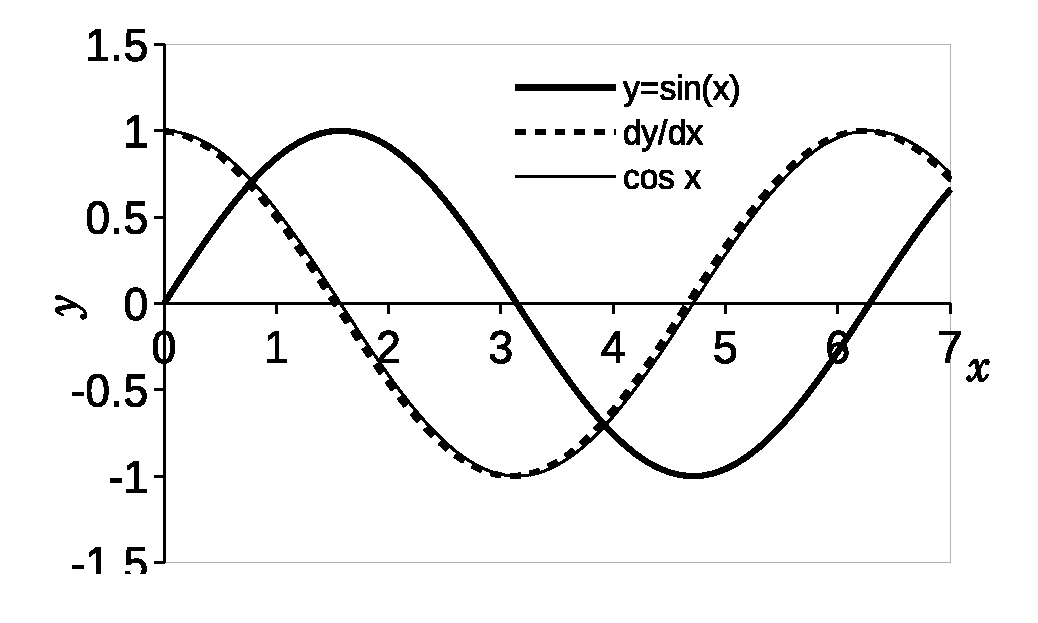
\includegraphics[width=8cm]{diffsin.eps}
    \caption{$y=\sin x$(太い実線)とその数値微分(点線), そして$y=\cos x$ (細い実線)
のグラフ。$x$の刻みは0.1。刻みをもっと小さくすると, 
$y=\sin x$の数値微分と$y=\cos x$はもっと近くなる。}\label{fig:diffsin}
\end{figure}

なんとびっくり! 上の問で, $\sin x$の数値微分は, $\cos x$のグラフに
ぴったり重なるではないか! つまり, $(\sin x)'=\cos x$なのだ!

\begin{q}\label{q:trig_numericdiff_cos} 表計算ソフトを用いて, 
\begin{enumerate}
\item $y=\cos x$のグラフを, $0\leq x \leq 7$の範囲で描け。
\item それを数値微分し, 結果をグラフに描け。
\item $y=-\sin x$のグラフに描け。
\end{enumerate}
$x$の刻みは0.1程度でOK。(1), (2), (3)のグラフは重ねて描くこと。
結果は\fref{fig:diffcos}のようになるはず。
\end{q}

\begin{figure}[h]
    \centering
    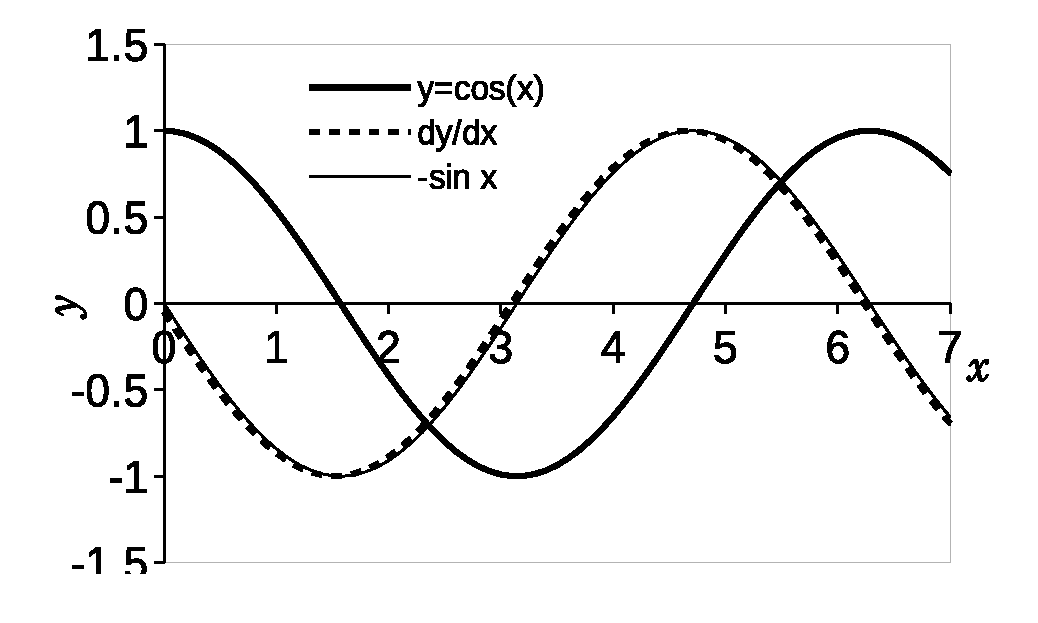
\includegraphics[width=8cm]{diffcos.eps}
    \caption{$y=\cos x$(太い実線)とその数値微分(点線), そして$y=-\sin x$ (細い実線)
のグラフ。$x$の刻みは0.1。刻みをもっと小さくすると, 
$y=\cos x$の数値微分と$y=-\sin x$はもっと近くなる。}\label{fig:diffcos}
\end{figure}

なんとまたびっくり! 上の問で, $\cos x$の数値微分は, $-\sin x$のグラフに
ぴったり重なるではないか! つまり, $(\cos x)'=-\sin x$なのだ!\mv

では$\tan x$の導関数は? $\tan x=\sin x/\cos x$に\pref{eq:difdiv}の\eref{eq:difdiv}をあてはめればよい。
すなわち, $v=\sin x$, $u=\cos x$として, 
\begin{eqnarray}
(\tan x)'&=&\Bigl(\frac{v}{u}\Bigr)'=\frac{v'u-vu'}{u^2}\nonumber\\
&=&\frac{(\sin x)'\,\cos x-\sin x\,(\cos x)'}{\cos^2x}\nonumber\\
&=&\frac{\cos x\,\cos x-\sin x\,(-\sin x)}{\cos^2x}\nonumber\\
&=&\frac{\cos^2 x+\sin^2 x}{\cos^2x}=\frac{1}{\cos^2 x}\label{eq:difftan}
\end{eqnarray}
となる。以上をまとめると, 
\begin{eqnarray}
(\sin x)'&=&\cos x\label{eq:diff_sinx}\\
(\cos x)'&=&-\sin x\label{eq:diff_cosx}\\
(\tan x)'&=&\frac{1}{\cos^2 x}\label{eq:diff_tanx}
\end{eqnarray}
である。この3つの公式は必ず記憶しよう。

\begin{faq}{\small\textgt{$\cos x$を微分する問題で, $\cos x=-\sin x$と書いたら
不正解になりました。なぜ?}
... 君は微分する前の関数と微分した後の関数を等号で結んで
しまっています。$(\cos x)'=-\sin x$と書くべきなのです。}\end{faq}

\begin{faq}{\small\textgt{でも, 答えは合っているからよくないですか?}
... その等式に$x=0$を代入してご覧。$1=0$になっちゃうよ。
それでもいいの?}\end{faq}

ここで, \eref{eq:diff_sinx}に$x=0$を代入すると, その値は$\cos 0=1$となる。
微分係数は, その関数のグラフの接線の傾きでもあるから, $y=\sin x$のグラフ, 
つまり, \pref{fig:sin}の図\ref{fig:sin}において, $x=0$での接線の傾きは1である。

\eref{eq:diff_cosx}に$x=0$を代入してみると, $-\sin 0=0$となる。
つまり, $y=\cos x$のグラフ, つまり, 図\ref{fig:cos}は, 
$x=0$での接線の傾きは0, つまりそこでグラフは平坦に
なることがわかる(実際, 図\ref{fig:cos}でもそうなっている)。

\eref{eq:diff_tanx}に$x=0$を代入してみると, $1/\cos^2 0=1$となる。
つまり, $y=\tan x$のグラフ, つまり, 図\ref{fig:tan}は, 
$x=0$で接線の傾きは1である。\hv

\eref{eq:diff_sinx}〜\eref{eq:diff_tanx}と, 
微分のいくつかの公式を組み合わせれば, 三角関数を含むいろんな関数を微分できる。

\begin{exmpl} 
  \begin{eqnarray}(\cos 3x)'=(-\sin 3x)(3x)'=-3\sin 3x\end{eqnarray}
  ↑ $\cos x$と$3x$の合成関数の微分。
\begin{eqnarray}(\sin^3 x)'&=&\{(\sin x)^3\}'=3\{(\sin x)^2\}(\sin x)'\nonumber\\
                             &=&3\sin^2x\,\cos x\end{eqnarray}
  ↑ $x^3$と$\sin x$の合成関数の微分。
\begin{eqnarray}(x^2\sin 3x)'&=&(x^2)'\sin 3x+x^2(\sin 3x)'\nonumber\\
                               &=&2x\sin 3x+x^2(3\cos 3x)\nonumber\\
                               &=&2x\sin 3x+3x^2 \cos 3x
\end{eqnarray}
  ↑ $x^2$と$\sin 3x$の積の微分。
(例おわり)\end{exmpl}\mv

\begin{exmpl} $f(x)=x^3\cos^2 3x$を微分してみよう。
$f(x)$を$x^3$と$\cos^2 3x$の積とみて, 積の微分の公式より, 
\begin{eqnarray*}f'(x)=(x^3)'\cos^2 3x + x^3\{(\cos^2 3x)'\}\end{eqnarray*}
右辺第一項の中の$(x^3)'$は$3x^2$である。右辺第二項の中の$(\cos^2 3x)'$は, $\cos 3x$
の2乗の微分とみなして合成関数の微分の公式を使えば, $2 \cos 3x\, (\cos 3x)'$となる。
$(\cos 3x)'$は, $3x$をひとつの変数とみなして合成関数の微分の公式により, $-3\sin 3x$となる。
これらをぜんぶ元に組み合わせれば, 
\begin{eqnarray*}f'(x)=3x^2\cos^2 3x - 6x^3\ \cos 3x\,\sin 3x\end{eqnarray*}
(例おわり)\end{exmpl}\mv

\begin{q}\label{q:trig_diff0} 次の関数を微分せよ。
\begin{edaenumerate}<3>
\item $\cos x$
\item $\tan x$
\item $\sin 2x$
\item $x \cos x$
\item $\cos^2 x$
\item $\cos x^2$
\end{edaenumerate}\end{q}
\mv

\begin{q}\label{q:trig_symmetry} 「微分」の章で, 奇関数の導関数は
偶関数, 偶関数の導関数は奇関数であることを学んだ。三角関数の導関数に
ついてそれらが成り立っていることを確かめよ。と言っても, 「確かめた」
だけでは解答にならないよ! どのように確かめたかを, ちゃんと書くこと。
\end{q}
\mv


\section{極座標}\label{sect:polar_coord_2D}

\begin{q}\label{q:trig_2Dpolar0} $xy$平面上の任意の点P$(x, y)$について, 原点からの距離を$r$とする。
つまり$r=\sqrt{x^2+y^2}$とする。点Pは, 原点を中心とする半径$r$の円周上
にある。いま, $\theta$を$x$軸から点Pまでの左回りの角とすると, 
\begin{eqnarray}\begin{cases}
x = r \cos \theta\label{eq:2Dpolar}\\
y = r \sin \theta
\end{cases}\end{eqnarray}
と書けることを示せ(図\ref{fig:2D_polar_coordinate})。
\begin{figure}[h]
    \centering
    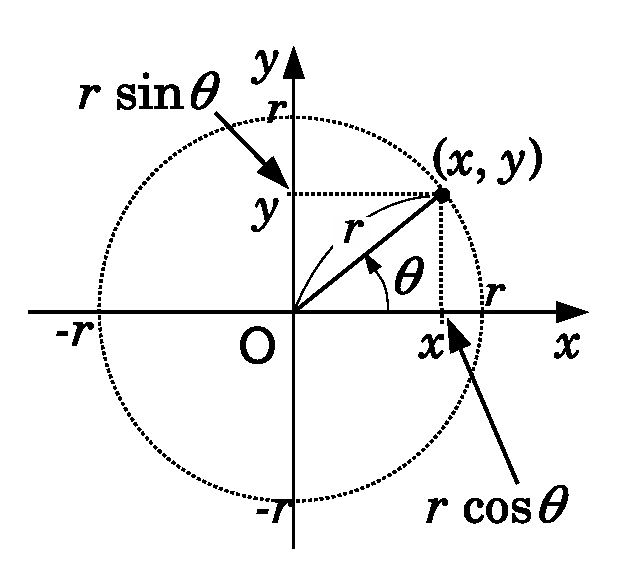
\includegraphics[width=5cm]{2D_polar_coordinate.eps}
    \caption{極座標の説明図。図\ref{fig:unit_circle}を$r$倍に拡大したものと考えてもよい。}\label{fig:2D_polar_coordinate}
\end{figure}
\end{q}

上のように, 平面上の点の位置を, 原点からの距離$r$と$x$軸からの角$\theta$であらわすことを, 
\underline{極座標} \index{きょくざひょう@極座標} (polar coordinate)と呼ぶ。それに対して, 
君が慣れ親しんだ, $x$軸と$y$軸のそれぞれに沿った成分の大きさであらわす$(x, y)$のようなあらわしかたを, 
\underline{デカルト座標} \index{でかるとざひょう@デカルト座標}
と呼ぶ\footnote{ちなみに3次元空間の点についても「極座標」は存在する(大学数学の範囲)。}。

\begin{q}\label{q:trig_2Dpolar1} 以下の
デカルト座標を極座標に, 極座標をデカルト座標に書き換えよ:
\begin{enumerate}
\item (1,1)
\item ($-\sqrt{3}$,1)
\item (2,3)  ヒント: $\theta=\arctan(3/2)$。電卓使用。
\item $r=2,\,\, \theta=\pi/3$
\item $r=3,\,\, \theta=$10°  ヒント: 電卓使用
\end{enumerate}\end{q}
\mv


\section{単振動}

ばねに吊るされた重りの上下運動や, 振り子の左右運動など, 世の中には
周期的に振動する現象が多くある。中でも, 時刻$t$での物体の位置$x(t)$
が以下のような式:
\begin{eqnarray}
x(t)=x_0\cos(\omega t + \delta)\label{eq:trig_harmonic_oscilation}
\end{eqnarray}
であらわされる場合, その振動運動を単振動\index{たんしんどう@単振動}という。
ここで$x_0, \omega, \delta$はいずれも$t$によらない適当な定数であり, $x_0>0$とする。
$x_0$を振幅と呼び, $\omega$を\underline{角速度}\index{かくそくど@角速度}
と呼ぶ。

\begin{q}\label{q:trig_osci} 部屋の天井からバネをつるし, その末端に重りをつけて, つりあいの位置に
静止させる。この位置を原点とし, バネに沿って上向きに$x$軸を考えよう。
つりあいの位置から重りを$x_0$だけ持ち上げて静かに離すと, 重りは上下に
振動運動をする。そのとき重りの運動の様子は, 次式で表現される
\footnote{その理由は物理学で学ぶだろう。角速度$\omega$が, 
重りの質量とバネの強さで決まることも学ぶだろう。なお, このような
運動が実現するには, 空気抵抗が無視でき, $x_0$がバネの長さに
比べて十分に0に近いことが必要である。}:
\begin{eqnarray}x(t)=x_0\cos\omega t\end{eqnarray}
ここで, $t$は, 重りを離してから経過した時間。$x(t)$は, 時刻$t$における
重りの位置である。
\begin{enumerate}
\item この運動の周期を, $\omega$を使ってあらわせ。
\item 時刻$t$における速度を求めよ。
\item 時刻$t$における加速度を求めよ。
\item 振動の振幅が変わらないままで$\omega$が2倍になると, 速度や加速度の最大値はそれぞれ何倍になるか? 
\end{enumerate}\end{q}
\vv


\section{三角関数の合成}

三角関数には他にも公式がたくさんある。それらを暗記する必要はないけれど, 
自力で導出できるようにはなっておこう。そうすれば, たとえ忘れても, 
必要に応じて思い出して活用できるだろう。\\

$a, b$を任意の実数として, 
\begin{eqnarray}a \sin x + b \cos x\label{eq:trigsynth1}\end{eqnarray}
という形の式を, 適当な実数$A, p$を使って(ただし$0\leq A$, $0\leq p<2\pi$とする)
\begin{eqnarray}A \sin (x + p)\label{eq:trigsynth2}\end{eqnarray}
という形の式にすることを\underline{三角関数の合成}\index{さんかくかんすうのごうせい@三角関数の合成}という。その方法を以下に述べる:

まず, \eref{eq:trigsynth2}は, 加法定理(\pref{eq:add_sin2}の\eref{eq:add_sin2})より, 次式のように変形できる:
\begin{eqnarray*}
A \sin (x + p)&=&A\{\sin x \cos p+\cos x \sin p\}\\
&=&A\cos p\sin x +A\sin p \cos x 
\end{eqnarray*}
これが\eref{eq:trigsynth1}と等しくなるには, 
\begin{eqnarray}\begin{cases}
a = A \cos p\label{eq:trigsynth3}\\
b = A \sin p
\end{cases}\end{eqnarray}
であればよい。これは\eref{eq:2Dpolar}とよく似ている。
すなわち, $xy$平面上で$(a, b)$という座標で表される点を極座標で表したときの
$r$を$A$とし, $\theta$を$p$とすればよい。

\begin{exmpl} $\sin x + \cos x$について, 三角関数の合成をしよう。
この場合, $a=b=1$である。点$(1, 1)$の極座標は, $r=\sqrt{2}$, $\theta=\pi/4$である。
従って以下のようになる:
\begin{eqnarray*}
\sin x+\cos x=\sqrt{2}\,\sin \bigl(x+\frac{\pi}{4}\bigr)
\end{eqnarray*}
実際, 右辺の$\sqrt{2}\sin (x+\pi/4)$を加法定理で展開してみると, 
\begin{eqnarray*}
\sqrt{2}\,\sin (x+\frac{\pi}{4}) &=& \sqrt{2}\,\bigl(\sin x \, \cos \frac{\pi}{4} + \cos x \, \sin \frac{\pi}{4}\bigr)\\
&=& \sqrt{2}\,\bigl(\frac{\sqrt{2}}{2} \sin x + \frac{\sqrt{2}}{2} \cos x\bigr)\\
&=& \sin x + \cos x
\end{eqnarray*}
となり, 左辺に等しくなっている。\\
\end{exmpl}

\begin{exmpl} 
\begin{enumerate}
\item $\sin x-\cos x=\sqrt{2}\sin (x-\pi/4)$
\item $\sqrt{3}\sin x+\cos x=2\sin(x+\pi/6)$
\item $\sin x-\sqrt{3}\cos x=2\sin(x-\pi/3)$
\end{enumerate}\end{exmpl}
\mv
三角関数の合成は, 物理学で出てくる「波の干渉」などで, 
波長の等しい正弦波形の重ねあわせをするときに使う。\mv


\section{積和公式と和積公式}

加法定理, すなわち\pref{eq:add_sin1}の\eref{eq:add_sin1}, \eref{eq:add_sin3}より, 
\begin{eqnarray*}
\cos(\alpha + \beta)=\cos\alpha \cos\beta - \sin\alpha \sin\beta\\
\cos(\alpha - \beta)=\cos\alpha \cos\beta + \sin\alpha \sin\beta
\end{eqnarray*}
これらの両辺を加えたり引いたりすると, 
\begin{eqnarray}
&&\cos(\alpha + \beta)+\cos(\alpha - \beta)=2\cos\alpha \cos\beta\label{eq:waseki1}\\
&&\cos(\alpha + \beta)-\cos(\alpha - \beta)=-2\sin\alpha \sin\beta\label{eq:waseki2}
\end{eqnarray}
となる。すなわち, 
\begin{eqnarray}
\cos\alpha \cos\beta=\frac{\cos(\alpha + \beta)+\cos(\alpha - \beta)}{2}\label{eq:sekiwa1}\\
\sin\alpha \sin\beta=\frac{\cos(\alpha - \beta)-\cos(\alpha + \beta)}{2}\label{eq:sekiwa2}
\end{eqnarray}
となる。一方, \pref{eq:add_sin2}の\eref{eq:add_sin2}, \eref{eq:add_sin4}より, 
\begin{eqnarray*}
\sin(\alpha + \beta)=\sin\alpha \cos\beta + \cos\alpha \sin\beta\\
\sin(\alpha - \beta)=\sin\alpha \cos\beta - \cos\alpha \sin\beta
\end{eqnarray*}
これらの両辺を加えると,
\begin{eqnarray}
\sin(\alpha + \beta)+\sin(\alpha - \beta)=2\sin\alpha \cos\beta\label{eq:waseki3}
\end{eqnarray}
となる。すなわち, 次式が成り立つ:
\begin{eqnarray}
\sin\alpha \cos\beta=\frac{\sin(\alpha + \beta)+\sin(\alpha - \beta)}{2}\label{eq:sekiwa3}
\end{eqnarray}

\eref{eq:sekiwa1}, \eref{eq:sekiwa2}, \eref{eq:sekiwa3}は, 2つの三角関数の積を, 
2つの三角関数の和に変換する公式であり, 「積和公式\index{せきわこうしき@積和公式}」と呼ばれる。

また, \eref{eq:waseki1}において, 
\begin{eqnarray}
\alpha+\beta=A\label{eq:alphabetaAB1}\\
\alpha-\beta=B\label{eq:alphabetaAB2}
\end{eqnarray}
とすれば, 
\begin{eqnarray}
\cos A+\cos B=2\cos\alpha \cos\beta\label{eq:waseki15}
\end{eqnarray}
となる。ところが, \eref{eq:alphabetaAB1}+\eref{eq:alphabetaAB2}より, $2\alpha=A+B$。
\eref{eq:alphabetaAB1}$-$\eref{eq:alphabetaAB2}より, $2\beta=A-B$。従って, 
\begin{eqnarray*}
\alpha=\frac{A+B}{2},\,\,\,\,\,
\beta=\frac{A-B}{2}
\end{eqnarray*}
なので, \eref{eq:waseki15}は, 
\begin{eqnarray}
\cos A + \cos B = 2\cos\frac{A+B}{2} \cos\frac{A-B}{2}\label{eq:waseki17}
\end{eqnarray}
となる。同様に, \eref{eq:waseki2}, \eref{eq:waseki3}より, 
\begin{eqnarray}
&&\cos A - \cos B = -2\sin\frac{A+B}{2} \sin\frac{A-B}{2}\label{eq:waseki27}\\
&&\sin A + \sin B = 2\sin\frac{A+B}{2} \cos\frac{A-B}{2}\label{eq:waseki37}
\end{eqnarray}
となる。\eref{eq:waseki17}, \eref{eq:waseki27}, \eref{eq:waseki37}は, 2つの三角関数の和(や差)を, 
2つの三角関数の積に変換する公式であり, 「和積公式\index{わせきこうしき@和積公式}」と呼ばれる。
\mv

和積公式は, 物理学で出てくる「うなり」という現象などで, 
わずかだけ波長が違う正弦波の重ねあわせをするときに使う。\hv

%\begin{q}\label{q:trigonometry_English} 以下の言葉を英訳せよ:
%\begin{edaenumerate}<3>
%\item ラジアン
%\item 単位円
%\item 極座標
%\end{edaenumerate}
%\end{q}\mv

\section*{演習問題}
\mv

\begin{exq}\label{q:trig_arcgraph}  
\begin{enumerate}
\item $y=\arccos x$, $y=\arcsin x$, $y=\arctan x$のそれぞれの導関数を求めよ。
\item $y=\arccos x$, $y=\arcsin x$, $y=\arctan x$
のそれぞれのグラフを描け。ヒント: 定義を再確認し, $y$のとり得る値の範囲に注意。
\end{enumerate}
\end{exq}
\mv

\begin{exq}\label{q:trig_sin_approx} 
\begin{enumerate}
\item 次式を証明せよ
\begin{eqnarray}
\lim_{\theta\rightarrow0}\frac{\sin \theta}{\theta}=1
\end{eqnarray}
ヒント: 高校数学の教科書に載っている。
\item それを用いて, $(\sin x)'=\cos x$を証明せよ。ヒント: \eref{eq:waseki37}。
\item それを用いて, $(\cos x)'=-\sin x$を証明せよ。ヒント: \eref{eq:trig_sinx_2pi}。
\end{enumerate}
\end{exq}
\hv

\section*{問題の解答}
(以下, ?は「解答丸写し」を防ぐための伏せ字。自分で考えよう!) 

\noindent{\textbf{答}}\ref{q:trig_Pitag}\
\begin{enumerate}
\item 角Aは共通で等しく, かつ, A以外の1つの角が直角で等しい。2つの角が等しいので相似。
\item △ABCと△ACDは相似なので, \\AB:AC=AC:AD。従って, AC$^2$=AB$\times$AD。
\item 角Bは共通で等しく, かつ, B以外の1つの角が直角で等しい。2つの角が等しいので相似。
\item △ABCと△CBDは相似なので, \\AB:BC=BC:BD。従って, BC$^2$=AB$\times$BD。
\item (2)よりAD=AC$^2$/AB。(4)よりBD=BC$^2$/AB。これをAB=AD+BDに代入して, \\
AB=AC$^2$/AB+BC$^2$/AB。\\両辺にABを掛けて, \eref{eq:pitagorus_0}を得る。
\end{enumerate}
\mv

\noindent{\textbf{答}}\ref{q:trig_rad_def} 
「ラジアン」とは, 角の大きさを, その角が半径1の円を切り取る扇型の弧の長さで表したもの。\\
ラジアンで表された数値=度で表された数値$\times \pi/180$
\mv

\noindent{\textbf{答}}\ref{q:trig_deg2rad} 
(1) $\pi/2\,$ (2) $\pi/4\,$ (3) $\pi\,$ (4) $\pi/6\,$ (5) $\pi/180$
\mv

\noindent{\textbf{答}}\ref{q:trig_rad2deg} 
(1) $180^{\circ}\,$ (2) $60^{\circ}\,$ (3) $360^{\circ}$ (4) $45^{\circ}\,$ (5) $180^{\circ}/\pi$
\mv

\noindent{\textbf{答}}\ref{q:trig_rad2rad}  (1) $\pi\,$ (2) $\pi\,$ (3) $0$
\mv


\noindent{\textbf{答}}\ref{q:Bitterrich}
\begin{enumerate}
\item 君の目を中心として, 腕の長さ($l$)を半径とする円において, 親指の幅$a$が切り取る弧の角度は, $\theta \fallingdotseq a/l$となる。
\item 君の目を中心として, 半径$R$の円において, 胸高直径$d$の木の幹が切り取る弧の角度は, $d/R$である。幹が親指にちょうどぴったり隠れるとき, 
この角度と前問の角度が等しくなるから, $\theta=d/R$。よって, $d=R\theta$
\item 前問より, 親指に隠れない木は, すべて半径$R$の円内にあり, かつ, 半径$R$の円内にある木はどれも親指からはみだして見える。従って, 
$N$は君の立ち位置を中心とする半径$R=d/\theta$の円内の木の本数である。
\item $A=\pi R^2$は自明。この円内にある木の胸高断面積の合計は, それぞれの木の胸高断面積$\pi (d/2)^2$と$N$の積だから, $B=N\pi d^2/4$
\item 前問より, 
\[\frac{B}{A}=\frac{N\pi d^2/4}{\pi R^2}\]
ここで, (2)より$d=R\theta$とすれば, この上の式の右辺は, 
\[=\frac{N\theta^2}{4}\]
となる。
\item $a=2$ cm, $l=60$ cmのとき, $\theta \fallingdotseq a/l= 1/30$。これと$N=10$を上の式に代入して, $B/A=0.0028$。
(地表面の0.28パーセントが木の幹で占められている。)
\item \eref{eq:Bitterrich_5}は, 木の太さ(胸高直径)$d$に依存しない。従って, この方法は, どんな太さの木からなる林についても有効である。
\item 太さ$d_1, d_2, ..., d_n$の木が混在しているとし, 親指に隠れない本数は, 太さ$d_k$の木について$N_k$本だったとする($1\leq k\leq n$)。
\eref{eq:Bitterrich_5}より, 太さ$d_k$の木に関する単位面積当たりの胸高断面積$C_k$は, $C_k=N_k\theta^2/4$となる。全ての木に関する, 
単位面積当たりの胸高断面積$C$は, $C_1+C_2+...+C_n=(N_1+N_2+...+N_n)\theta^2/4=N\theta^2/4$となり, 結局, 
$N=N_1+N_2+...+N_n$, すなわち, さまざまな太さの木をぜんぶひとまとめにして親指に隠れない本数を数えたときの値
だけで決まる。従って, さまざまな太さの木が混在する状況でも, この方法は有効である。
\end{enumerate}
\mv

\noindent{\textbf{答}}\ref{q:trig_unitC} 
半径1の円。
\mv

\noindent{\textbf{答}}\ref{q:trig_sincos_def} 略 (本文に書いてある)。
\mv

\noindent{\textbf{答}}\ref{q:trig_sincos2} 
定義より$(\cos\theta,\, \sin\theta)$で表される点Pは$xy$平面上の原点
を中心とする単位円の上の, いかなる点もとりうる。よって, $\cos \theta$すなわちPの$x$座標と, 
$\sin \theta$すなわちPの$y$座標は, $-1$から$1$の範囲のどんな値もとりうる。
しかし, 点Pはこの単位円上以外の点はとらない。従って$\cos \theta$も$\sin \theta$も, 
$-1$より小さくなったり$1$より大きくなったりはしない。\mv

\noindent{\textbf{答}}\ref{q:trig_sincos6} \\
\begin{tabular}{rrrr} \toprule
角         &  sin                      & cos                     & tan \\ \midrule
$0^{\circ}$   &   0                     &   1                      &   0 \\
$30^{\circ}$ & $1/2$                     & $\sqrt{3}/2$            & $1/\sqrt{3}$\\
$45^{\circ}$ & $1/\sqrt{2}$             &  $1/\sqrt{2}$            &  $1$\\
$60^{\circ}$ & $\sqrt{3}/2$             &  $1/2$                    &  $\sqrt{3}$\\
%$75^{\circ}$ & $(\sqrt{6}+\sqrt{2})/4$  & $(\sqrt{6}-\sqrt{2})/4$  &  $2+\sqrt{3}$ \\  
$90^{\circ}$ & $1$                       &  $0$                      &  解なし\\
$120^{\circ}$ & $\sqrt{3}/2$            &  $-1/2$                   &  $-\sqrt{3}$\\
%$150^{\circ}$ & $1/2$                    &  $-\sqrt{3}/2$           &  $-1/\sqrt{3}$\\
$180^{\circ}$ & $0$                      &  $-1$                     &  $0$\\
$270^{\circ}$ & $-1$                    &  $0$                      & 解なし\\
$-30^{\circ}$ & $-1/2$                  &  $\sqrt{3}/2$            & $-1/\sqrt{3}$\\
$\pi/6$       & $1/2$                   &  $\sqrt{3}/2$            & $1/\sqrt{3}$\\
$\pi/4$       & $1/\sqrt{2}$            &  $1/\sqrt{2}$            & $1$\\
$\pi/3$       & $\sqrt{3}/2$             &  $1/2$                    &  $\sqrt{3}$\\
$1^{\circ}$  & $0.017\cdots$  & $0.999\cdots$ & $0.017\cdots$ \\ 
%1            & $0.841\cdots$  & $0.540\cdots$ & $1.557\cdots$ \\ 
%0.1          & $0.099\cdots$  & $0.995\cdots$ & $0.100\cdots$ \\ 
1            & $0.?41\cdots$  & $0.?40\cdots$ & $1.??7\cdots$ \\ 
0.1          & $0.??9\cdots$  & $0.9?5\cdots$ & $0.1??\cdots$ \\ 
0.01         & $0.010\cdots$  & $0.999\cdots$  & $0.010\cdots$ \\ \bottomrule
\end{tabular}\\
\mv

%\noindent{\textbf{答}}\ref{q:trig_sincos3} 略。\mv

\noindent{\textbf{答}}\ref{q:trig_sincos4}
$n\pi$ラジアンの角は, $n$が偶数のときは0ラジアンの角と同じであり, 
$n$が奇数のときは$\pi$ラジアンの角と同じである。従って, 単位円上で, 
$x$軸から$n\pi$ラジアンの角にある点Pの座標は, $n$が偶数のときは$(1, 0)$であり, 
$n$が奇数のときは$(-1, 0)$である。いずれのときも, その$y$座標は0である。従って$\sin n\pi=0$。
同様の考察で点Pの$x$座標を考えると, $n$が偶数のときは1, $n$が奇数のときは$-1$。これは
$(-1)^n$と統一的に表現できる。従って, $\cos n\pi=(-1)^n$。\mv

\noindent{\textbf{答}}\ref{q:trig_tan}
$\tan^2\theta=\sin^2\theta/\cos^2\theta$だから, 
\begin{eqnarray*}
&&1+\tan^2\theta=1+\frac{\sin^2\theta}{\cos^2\theta}=\frac{\cos^2\theta+\sin^2\theta}{\cos^2\theta}=\frac{1}{\cos^2\theta}
\end{eqnarray*}
また, $\cos(-\theta)=\cos\theta$, $\sin(-\theta)=-\sin\theta$より, 
\begin{eqnarray*}
&&\tan(-\theta) = \frac{\sin(-\theta)}{\cos(-\theta)} = \frac{-\sin\theta}{\cos\theta}=-\tan\theta
\end{eqnarray*}
また, 
\begin{eqnarray*}
&&\tan(\theta+\pi) = \frac{\sin(\theta+\pi)}{\cos(\theta+\pi)}
= \frac{-\sin \theta}{-\cos \theta}
= \frac{\sin \theta}{\cos \theta}
=\tan\theta
\end{eqnarray*}
\mv

\noindent{\textbf{答}}\ref{q:trig_evenodd}\\
\eref{eq:trig_cos_even}から, $\cos \theta$は偶関数。\\
\eref{eq:trig_sin_odd}から, $\sin \theta$は奇関数。\\
\eref{q:trig_tan_minus}から, $\tan \theta$は奇関数。
\mv

\noindent{\textbf{答}}\ref{q:trig_kahouteiri}  略(誘導に従う)。
\mv

\noindent{\textbf{答}}\ref{q:trig_kahouteiri2} 
\begin{enumerate}
\item 略。前問で$\beta$をあらたに$-\beta$と置き直せばよい(実際に計算してみよ)。
\item 略。前問で$\beta$をあらたに$-\beta$と置き直せばよい(実際に計算してみよ)。
\item $\cos (\alpha+\beta)=\cos\alpha\cos\beta-\sin\alpha\sin\beta$において, 
$\beta=\alpha$とおけば, $\cos 2\alpha=\cos^2\alpha-\sin^2\alpha$。また, 
$\cos^2\alpha+\sin^2\alpha=1$より, $\sin^2\alpha=1-\cos^2\alpha$。これを
使って上の結果の$\sin^2\alpha$を消去すれば, $\cos 2\alpha=2\cos^2\alpha-1$。
同様に, $\cos^2\alpha=1-\sin^2\alpha$を使って上の結果の$\cos^2\alpha$を
消去すれば, $\cos 2\alpha=1-2\sin^2\alpha$。
\item $\sin (\alpha+\beta)=\sin\alpha\cos\beta+\cos\alpha\sin\beta$において, 
$\beta=\alpha$とおけば, $\sin 2\alpha=2\sin\alpha\cos\alpha$。
\end{enumerate}
\mv


\noindent{\textbf{答}}\ref{q:trig_sincos5} 
\begin{enumerate}
\item 式(\ref{eq:cos2_2})より, $\cos 2\alpha = 2\cos^2 \alpha - 1$。これを変形して与式を得る。
\item 式(\ref{eq:cos2_3})より, $\cos 2\alpha = 1 - 2\sin^2 \alpha$。これを変形して与式を得る。
\end{enumerate}
\mv



\noindent{\textbf{答}}\ref{q:trig_singraph0} 
(1)(2)(3)は, 図\ref{fig:sin}, 図\ref{fig:cos}, 図\ref{fig:tan}参照。
(4)は, 図\ref{fig:sin}を横方向に半分に縮めたもの(グラフの縮小)。
\mv

\noindent{\textbf{答}}\ref{q:trig_singraph1}  
\begin{enumerate}
\item $\sin x$は常に実数なので, その二乗である$\sin^2 x$は常に0以上。
\item 常に$-1 \le \sin x \le 1$なので, $\sin^2 x \le 1$。
\item $x=0$のとき$y=\sin^2 x=0$。従って原点を通る。
\item $f(x)=\sin^2x$とすると, $f(-x)=\sin^2(-x)=(-\sin x)^2=\sin^2x=f(x)$。従って偶関数。
\item 式(\ref{eq:sin_pow2})より, この関数のグラフは, 関数$y=\cos 2x$のグラフを$y$軸方向に$-1/2$倍して$y$軸方向に$1/2$移動したものだ。
そのグラフは, 図\ref{fig:sin_square}参照
\end{enumerate}

\mv
\noindent{\textbf{答}}\ref{q:trig_triang_sincos0}  単位円上に, $x$軸から角$\theta$の位置に点Pをとる。点Pから$x$軸におろした垂線の
足を点Qとする。三角形OPQは, 直角三角形OABと相似である。OP$=1$なので, 三角形OPQの
OA倍が三角形OABになる。
\begin{enumerate}
\item PQ$=\sin \theta$なので, AB=PQ$\times$OA=OA$\,\sin \theta$。よって$\sin\theta=$AB/OA。
\item OQ$=\cos\theta$なので, OB=OQ$\times$OA=OA$\,\cos \theta$。よって$\cos\theta=$OB/OA。
\item これらより, 
\begin{eqnarray*}\tan\theta=\frac{\sin\theta}{\cos\theta}=\frac{\text{AB/OA}}{\text{OB/OA}}=\frac{\text{AB}}{\text{OB}}\end{eqnarray*}
\end{enumerate}
\mv

\noindent{\textbf{答}}\ref{q:trig_triang_sincos1} \eref{eq:trig_defclassic_sin1}で, 
ABを高度, OAを斜距離と考えればよい。高度=100$\,\,$m$\times \sin($30度)=50$\,\,$m。
\mv

\noindent{\textbf{答}}\ref{q:trig_triang_sincos2} 高度=100$\,\,$m$\times \sin$(3度)。
関数電卓で計算すると, $\sin$(3度)$=0.05233595\cdots$なので,\\
高度=100$\,\,$~m$\times 0.05233595\cdots=5.233\cdots$~m。

一方, 3度$=\pi/60$ラジアンは, 0に近いので, 関数電卓を使わないでも, 
\begin{eqnarray*}
\sin(3\text{度})=\sin(\pi/60)\fallingdotseq\pi/60=0.05235986\cdots
\end{eqnarray*}
となる。従って, 高度$\fallingdotseq$100$\,\,$m$\times 0.05235986\cdots=5.235\cdots$m。
このように, 近似による誤差は, わずか2〜3$\,\,$mm程度である。
\vspace{0.3cm}

\noindent{\textbf{答}}\ref{q:trig_seigen} 
\begin{enumerate}
\item 直角三角形CBPで, $\text{BP=CB}\sin C=a\sin C$。
\item 三角形ABCについて, 底辺をCA$=b$, 高さをBPとすれば, 前問より, 
\begin{eqnarray*}
S=\frac{\text{CA}\times \text{BP}}{2}=\frac{ab\sin C}{2}
\end{eqnarray*}
\item 前小問によって, 「三角形の面積は, 2辺の長さ×それらが挟む角の正弦/2」
ということがわかった。これを, 辺CAと辺ABに適用すると\eref{eq:triangle_area22}
を得るし, 辺ABと辺BCに適用すると\eref{eq:triangle_area23}を得る。
\item \eref{eq:triangle_area1}〜\eref{eq:triangle_area23}より, 
\begin{eqnarray*}
S=\frac{ab\sin C}{2}=\frac{bc\sin A}{2}=\frac{ca\sin B}{2}
\end{eqnarray*}
これらに$2/(abc)$をかければ(いちばん左の$S$の項は落として), 
\begin{eqnarray*}
\frac{\sin C}{c}=\frac{\sin A}{a}=\frac{\sin B}{b}
\end{eqnarray*}
これらの逆数をとれば与式を得る。
\end{enumerate}


\noindent{\textbf{答}}\ref{q:trig_yogen} 
\begin{enumerate}
\item 直角三角形CBPを考えればCP=BC$\cos C=a\cos C$。また, 
AP=$|$AC$-$CP$|$=$|b-a\cos C|$。
注: 絶対値は, Pが線分CAの外側にあるときに必要。
\item 直角三角形PABを考える。斜辺ABの長さは$c$。直角をはさむ2辺はAPとPBであり, 
前小問よりAP=$|b-a\cos C|$。また, PB=$a\sin C$。これらに三平方の定理を適用して
与式を得る。
\item 前小問の与式を展開すると,
\begin{eqnarray*}
c^2&=&a^2\sin^2 C+b^2+a^2\cos^2C-2ab\cos C\\
   &=&a^2(\sin^2 C+\cos^2C)+b^2-2ab\cos C\\
   &=&a^2+b^2-2ab\cos C\\
\end{eqnarray*}
%\item 略($\cos C=$の形に式変形するだけ)
\end{enumerate}
\mv

%\noindent{\textbf{答}}\ref{q:trig_yogen_pyutag} 略。\mv

\noindent{\textbf{答}}\ref{q:trig_area} 
\begin{eqnarray*}
&&(1)\,\,\,\,\,\cos\theta=\frac{a^2+b^2-c^2}{2ab}=\frac{21}{24}=\frac{7}{8}\\
&&(2)\,\,\,\,\,\sin\theta=\sqrt{1-\cos^2\theta}=\sqrt{1-\bigl(\frac{7}{8}\bigr)^2}=\frac{\sqrt{15}}{8}\\
&&(3)\,\,\,\,\,S=\frac{ab\,\sin\theta}{2}=\frac{3\sqrt{15}}{4}\,\,\text{cm}^2
\end{eqnarray*}
注:(3)については, 必ず単位をつけること!
\mv



% 逆三角関数
\noindent{\textbf{答}}\ref{q:trig_arcsin} 
\begin{edaenumerate}
\item $\arctan 1=\pi/4$
\item $\arctan 0=0$
\item $\arccos 0.5=\pi/3$
\item $\arcsin (-0.5)=-\pi/6$
\item $\arctan 5=1.373\cdots$
\item $\arcsin 2$は存在しない。
\end{edaenumerate}
\mv

\noindent{\textbf{答}}\ref{q:trig_arcsin2}
 有効数字2桁で計算すればよい。関数電卓を使って, $\arctan\{(880-30)/12000\}\fallingdotseq0.071\text{ラジアン}=4.1$度
\mv


% 三角関数の微分

\noindent{\textbf{答}}\ref{q:trig_numericdiff_sin} 略 (プリントアウトせよ)。

\noindent{\textbf{答}}\ref{q:trig_numericdiff_cos} 略 (プリントアウトせよ)。

\noindent{\textbf{答}}\ref{q:trig_diff0}  
\begin{enumerate}
\item $-\sin {x}$
\item $1/\cos^2 x$
\item $2\cos{2x}$
\item $\cos{x}-x\sin{x}$
\item $-2\cos x\,\sin x$。または, $\sin$の倍角公\eref{eq:sin2a}を使って, $-\sin{2x}$としてもよい。
\item $-2x\sin{x^{2}}$
\end{enumerate}
\mv


% 極座標
\noindent{\textbf{答}}\ref{q:trig_2Dpolar0}  単位円上に, $x$軸から角$\theta$の位置に点P$_0$をとる。点P$_0$は線分OP上に
あり, かつ, OP$=r$, OP$_0=1$なので, 点Pの座標$(x, y)$は点P$_0$の座標$(\cos\theta, \sin\theta)$
の$r$倍。従って, $x=r\cos{\theta}$, \, $y=r\sin{\theta}$。
\mv

\noindent{\textbf{答}}\ref{q:trig_2Dpolar1} 
\begin{enumerate}
\item $r=\sqrt{1^{2}+1^{2}}=\sqrt{2},\,\, \theta=\pi/4$
\item $r=2,\,\, \theta=5\pi/6$
\item $r=\sqrt{2^2+3^2}=\sqrt{13},\,\, \theta=\arctan(3/2)=0.982\cdots$
\item $x=r\cos{\theta}=2 \times \cos(\pi/3) = 1$\\
       $y=r\sin{\theta}=2 \times \sin(\pi/3) = \sqrt{3}$\\
       $\therefore (1, \, \sqrt{3})$
\item 同様にして$(2.95\cdots, \, 0.520\cdots)$
\end{enumerate}
\mv

%
\noindent{\textbf{答}}\ref{q:trig_osci} 
\begin{enumerate}
\item $\cos$は$2\pi$を周期とする関数なので, $x_0\cos \omega t$は, $\omega t= 2\pi$になるときにもとに戻る。
従って, 運動の周期を$T$とすると, $\omega T=2\pi$。従って, $T=2\pi/\omega$である。
\item $(x_0\cos \omega t)'=-x_0\omega \sin{\omega t}$
\item $(x_0\cos \omega t)''=-x_0\omega^2 \cos{\omega t}$
\item 速度の最大値は$x_0\omega$, 加速度の最大値は$x_0\omega^2$なので, $\omega$が2倍になると, 
速度の最大値は2倍, 加速度の最大値は4倍になる。
\end{enumerate}

